\documentclass[11pt,a4paper,footinclude=true,headinclude=true, oneside]{scrbook}
\usepackage[T1]{fontenc} 	
\usepackage{graphicx}
\usepackage{lipsum}
\usepackage{tabu}
\usepackage{booktabs}
\usepackage[linedheaders,parts,pdfspacing]{classicthesis} % ,manychapters
%\usepackage[osf]{libertine}
\usepackage{amsthm}
\bibliographystyle{IEEEtran}

\begin{document}

\begin{titlepage}
   \begin{center}
       \vspace*{1cm}

        \begin{figure}[htbp]
            \centerline{
\includegraphics[scale=.5]{hs-hl.jpg}}
        \end{figure}
       \textbf{Drone Application in Precision Agriculture}
            
       \vspace{0.5cm}

       \textbf{Vytaras Juraska}

       \vfill
            
       \vspace{0.8cm}
            
       Electronics Engineering student of\\
       Hamm-Lippstadt Hochschule\\
            
   \end{center}
\end{titlepage}

%	\pagestyle{scrheadings}
%	\manualmark
%	\markboth{\spacedlowsmallcaps{\contentsname}}{\spacedlowsmallcaps{\contentsname}}
	
	\tableofcontents 

%	\automark[section]{chapter}
%	\renewcommand{\chaptermark}[1]{\markboth{\spacedlowsmallcaps{#1}}{\spacedlowsmallcaps{#1}}}
%	\renewcommand{\sectionmark}[1]{\markright{\thesection\enspace\spacedlowsmallcaps{#1}}}

    % use \cleardoublepage here to avoid problems with pdfbookmark
\chapter{Introduction}
	
Over the years, a lot of burning questions come up, which deducts how well and for how long the human race can survive for on the land, that we've got. There are many, still unsolved and exponentially growing issues, which we still have no solution to, but one of the biggest topics, which will most likely always be an important topic upon which we, as a humankind can improve - agriculture.
    
It is self explanatory, more people on earth, requires more food, more food - use more land. But land is not an endless resource, so what else can we do, to keep growing the quantity and quality of the food production, keeping in mind, that land is a precious resource, which we can not use for granted. Well this specific topic is expanded and still remains to be a very important subject 'till this day, called Precision Agriculture (PA).
    
    
\chapter{Definition of Precision Agriculture}
    
This specific topic analyses and develops the most efficient methods on how to monitor and reassure the quality, sustainability and protection of crops, soil and the environment surrounding the specific area of agriculture.
    
From simple humidity sensors, to whole autonomous drones collecting information and spraying various supportive chemicals aiding crops in the growth process, to even laser land leveling, to reassure as precisely flat as possible land - there are endless implementations in this field and since it is relatively new and still in constant development, various of new adaptations are arising each day.
    

\section{Technology}

Generally PA mostly uses technology, which are common in automation and robotics, such as geographic information systems, global positioning systems, remote sensing and various wireless network communication implementations.

Focusing on the less common technologies, which are purely created for PA, there are also many various methods of implementation, from different purposed software solutions to specific hardware systems. Just naming a few:

\begin{itemize}
    \item SmartNode - low cost software and hardware platform, which is used to monitor agriculture specific climate variables for optimal crop development (reference \cite{nunez_v_design_2017});
    \item Floratest - a digital tool, which estimates a plants state in several seconds without needing to inflict damage to the plant itself. The data used in this implementation is chlorophyll fluorescent induction, which is a property of plants light re-emission after being exposed to a bright light, the result - a graph of this specific signal. Surprisingly there are many areas of application for this device: quick estimate of plants vital activity after environmental hazards (like drought, frost, pesticide infection), quick detection of optimal doses of chemical fertilizers, quick detection of water pollution used by the plants and so on (reference \cite{palagin_data_2011}).
\end{itemize}

    
\section{Variables}

Properties, which are important in agriculture and their are as follows (reference \cite{lokhande_effective_2021}): 
\begin{itemize}
    \item Weather - specific crops perform better or worse on specific weathers. In order to maximise production, a prediction of the upcoming weather is carried out, after which a specific crop is seeded for the corresponding prediction;
    \item Soil - use of pesticides, sometimes ordinary constant crop growth in the same soil, many aspects impact the fertility of the soil, hence a careful selection of a crop in a specific soil has to be made;
    \item Crop cutting - with image processing it is possible to pinpoint which parts of the crops in the field are ready for cutting. There are cases, where crops grow unevenly, to maximise production specific crops are being cut only when they need to be cut;
    \item Pests management - various of aspects can control and predict which kind of pests have a chance of spread, pesticide chemicals are known to affect the organic structure of growing crops more or less, hence knowing for what pests to prepare for and only using what is necessary saves costs on supplies, ensures organic production and improves production quality overall;
    \item Intercropping - having the information about crop growth impacting properties can open up opportunities for successful intercropping, a method of growing more than one crop at the same time, in the same field. Since this method requires precise information, PA provides a possible better choice of crop.
\end{itemize}
Of course each PA product, each system has their own crucially important variables, for instance: temperature, solar radiation, humidity, soil moisture, wind and so on. But mainly, the  information collected is to fit one of these groups of information listed above, to find the most suitable crop or crops for a specific field, preparation for pesticides and overall health of the crop, to be as efficient in the production as possible. 
    
\section{Implementation}

For an example, in the United States one of the most common management schemes for creating a PA system goes as follows (reference \cite{tran_concept_nodate}):
\begin{itemize}
    \item Determine management zones for specific PA system implementation in each of the zones;
    \item Establish production goals;
    \item Sample and analyze the soil;
    \item Using the data of land preparation, varieties, fertilizers and other nutrient supplements decide upon the precise management to achieve desired production goal;
    \item Create maps of possible pest population and using principle methods, such as Integrated Pest Management, form an approach of how to deal with the pests of each zone in the field;
    \item Apply precision irrigation, an approach of providing the crop with a precisely measured amount of water and nutrients at the corresponding time, which creates the most optimal growing conditions for the crops;
    \item Form an automatic log and record tracking for all the data being constantly collected;
    \item Monitor and establish the whole PA system, evaluate the process and results and determine strengths and weaknesses of the system for future improvement.
\end{itemize}

While this is one of the standard procedures, there are other ways of implementation, for example The Australian Center of Precision Agriculture has its own crop management system implementation, which separates them into five main processes. 

Overall, there is no one true way of how to implement a PA system, each area is uniquely different from each other, hence the approach might always be different, but generally it is an integration of sensor systems and various technological approaches, which would focus on gaining the most suitable method of management for each specific piece of field.

\chapter{Drone Specification}

A drone is an unmanned aerial vehicle, which is generally a flying vehicle, which does not need to have a human on board to pilot it. Originally they were created and were most commonly used in military to perform various of tasks. Only about a decade ago drones became publicly available, where from that point on fields of drone application suddenly opened up to many various paths.

One of the fields, which just recently started to become more and more researched for drone application, is exactly in PA. In order to understand this specific field, it is useful to go through general understanding of common applications and characteristics of drones.

\section{Common Fields of Adaptation}

These days drones are really used in many fields: areal videography and photography, mapping and surveillance, delivery of goods and medical supplies, pipe inspections and even rescuing, but most importantly to this subject, it is already also used in agriculture (reference \cite{alwateer_enabling_2019}). 

Generally this specific piece of technology in theory has endless amounts of use cases. Taking a look at one of the most popular brands of drone manufacturing - DJI \footnote{www.dji.com}, their catalogue mostly focuses on video/photography, but they also have their line-ups for enterprise, with information about various fields of application, they have agriculture line-up, which focuses on spraying liquid on crops, mission planing line-up, which focuses on mapping out areas and packs other various features, they even have a developer line-up, where they provide an open-source drone, which a customer can program. Hence on the public market, there are many various of adaptations in drone industry, which any customer can easily buy right now.

\section{Safety}

There are various characteristics to consider, before flying a drone, not everywhere and not any homemade drone is available to be used. For starters, each country has their own aviation laws about drones, which are constantly changing, getting new additions, since the drone technology keeps getting improved very quickly \cite{alamouri_exploratory_2021}. 

Going further on, safety is not just a subject of law, but also the users concern. What will an autonomous drone do, if there is a person in front of it and it needs to occupy the space, where the person is standing, how users will communicate with the drones in real-time at dangerous situations \cite{doran_conceptual_2020} - a lot of unique topics are being investigated in the drone field.

One of the examples of how unstable the regulations are, according to an educational article
\cite{alamouri_exploratory_2021}, since 2013, there has been a very particular drone operating in Germany, which was 24.9 kg of weight, had a wing span of 3.6 meters and could reach altitudes up to 1000 meters, its name is "ALADINA" and getting the license to operate this specific drone was a constantly changing procedure, from requiring a big bulk of documents, having to call and inform about each flying session, and have people monitoring the procedure throughout the whole operation, went to much more softer regulations, soon after the regulations changed again and came back to the same strict laws as before.

To understand the current safety regulations, one has to keep track of global UAV regulations and location specific regulations, which in this case I will be considering EU regulations:

Global UAV regulations - the International Civil Aviation Organization
(ICAO\footnote{www.icao.int}) is the organisation, which is mostly responsible for handling global regulations of UAVs - directed by 193 national governments.

EU UAV regulations \cite{alamouri_exploratory_2021} - starting from early 2017, the European Aviation Safety Agency (EASA\footnote{www.easa.europa.eu}) released the first method
of regulating UAS by their maximum take-off mass (MTOM), the masses considered where: less than 5 kg, between 5 and 25 kg and over 25 kg. It was believed, that the risk is directly related to the potential kinetic energy of UAS, but in the same year, regulation for all of the UAS, regardless their MTOM, where created. Next year, the overall performance of civil aviation was improved, which resulted in a set of requirements for UAS technology and personnel, also demanding the involvement of remote pilots, when an operation with UAS is being performed. And finally, the newest bunch of regulations came in at 2020, where a big set of operation and technology regulations were formed: types of UAS operations were split into 3 categories, depending on the risk of the operation, correspondingly regulations and aviation authority involvement is proposed and also technical properties of each UAS were defined much more, introducing categories for each MTOM, defining their maximum allowed speed and so on (Figure \ref{categories}).

To sum all up, drone regulations and laws are very important to keep up with, since this technology is not well defined, constantly changing, and according to The CEO of the AscTec UAV (Unmanned Arial Vehicle) company, stresses that “legislation and policymaking is lagging way behind the technology” \cite{stocker_review_2017}.

\chapter{Drone Application to Precision Agriculture}

Having the information, that PA field is very progressive and has a tendency of adapting newest modern technology fairly quickly, as seen before, there is already a market for agriculture specific drones, which have various systems for taking care of the crops, like fluid spraying systems, with a very wide range of spray, while operating fully autonomously and collecting useful data of the environment, which is being instantly synced up with the cloud services. Drones in PA are useful for many reasons, some of the use case examples: detecting pest invasion at specific locations and using the correct pesticides for the specific pest invasion at the pin pointed location, where the pests are spreading, some drones are just fitted with remote sensing equipment and easily identify the driest sections of the field. The unique part of drone implementation, is that each drone can do crop maintenance tasks for each specific crop, and show almost any issue or potential threat to a specified crop. It is astonishing, that this technology is advancing and quickly adapting to specific use cases in such a quick rate. But to understand this blooming technology in specifically precision agriculture field, relevant information has to be analyzed.

\section{Classifications of Drones}

In the article \cite{Bacco_Smart_2018} a table of drone classifications in Precision Agriculture is introduced (Figure \ref{dronegroup}). The first layer in this table consists of general missions, performed in PA, while the second layer is expanding upon the first, introducing more specific roles.

For instance, one of the first level missions is treatment, specifying the activity of drones taking care of the crops in a physical application. This mission category splits to two roles, which are:
\begin{itemize}
    \item Spraying - the role of carrying specific liquid and spraying it on crops;
    \item Variable Rate Treatment - using a generated rate map, which specifies the amount of variable needed in each specific territory of the field. This can be applied to many variables - fertilizer, seed, pesticides.
\end{itemize}

There are three more categories: Intelligence/Reconnaissance, Transport and Communication. Each of these categories have roles defined in the same figure.
    
\section{Current Market and Features}

One of the drone manufacturers, which focuses on general consumer market - DJI, as mentioned before, have a lineup of drones adapted to agriculture. Their newest drone is DJI Agras T30\footnote{https://www.dji.com/lt/t30?site=brandsite\&from=nav}, it is equipped with 30 kg spraying tank and has the ability to spray liquid at the width of 9 meters, hence it can cover 40 acres per hour. This drone has obstacle detection and avoidance system implemented, has two cameras - in front and at the back, and has the ability to operate during the night. It can also be folded to 80 \% of its original size, which allows for easier compactness and transportation of the drone. Regarding its software, DJI have their route planning application, which helps specifying the path drones have to take. Other DJI agriculture products are inferior versions of this model.

SenseFly has their own lineup of PA drones - eBee Ag\footnote{https://www.sensefly.com/drone/ebee-ag/}. This one is meant for purely data collection and mission planning. Using their software and the specific camera sensor, eBee Ag flies autonomously through the field, lands where the user specifies, and in a couple of minutes this drone provides a series of maps of the field, which help with various applications. The official website states, that their technology creates maps with the precision of 2.5 cm. The most common application with this product, is generating variable rate treatment maps, a category, which is defined in the previous section. And the maximum coverage in one flight is 395 acres, since that is what the battery of the drone allows.

Hence, there are drone manufacturers, which have agriculture applications with ranging functionality and purpose in this field. Even if so far there are not a lot of choices for the a consumer to choose from, the current market is already covering the few important functionalities that the drones have to offer to agriculture in general.

\chapter{Drone communications in Precision Agriculture}

Truth be told, there are many various wireless functions and means of communications, that the main difficulty is rather not the available technology, but no standardised method, which would be widely implemented and accepted by many. Another issue, is that type of communication used is usually dependant on specific agricultural situations, hence to understand the market and availability of communications for PA in drone application, it is necessary to identify at least a couple of use cases and examples.

\section{ISOBUS future improvement}

A specific type of communication is created by Agricultural Electronic Foundation (AEF), which has international association with major industries and research centers, which are involved in technological improvement of agriculture machines and systems. AEF is creating a communication type, called ISOBUS, which is generally a mature standardisation, which is used by their associatives widely. But just recent announcements revealed, that AEF is working on time-sensitive networking, which would use Ethernet and BroadR-Reach technologies to create high speed communications from and to various agricultural machines, which are part of IoT devices.

\section{M2M/IOT Standards}

In a specific situations, where the working fields are fairly large, and an extensive cultivation process of grains has to be done, many huge machines and various other devices have to be working in parallel, real-time reliable communication is required. Hence, understanding the worst possible situation allows us to understand what to truly value in Farm Management Information Systems (FMIS).

The requirements for a reliable communication for clusters are: ability to exchange big amounts of data, maintain real-time communication and cooperation of big clusters of machinery, sharing data from sensors, maintain required communication speeds. Each situation demands specific values in these requirements, but in the current availability of communications in FMIS field, specifically Machine to Machine (M2M) Internet of Things (IoT) type of communications, it is easier to divide them by their range.

\subsection{IEEE}

Short-range: IEEE 802.15.4 - was intended for low-rate and Low-Power Wide-Area Network (LPWAN) applications. Its range is about 100 meters and it has very specific frequencies, upon which communication can be handled:

\begin{itemize}
    \item In Europe: 433 MHz, 868 MHz, 2.4 GHz;
    \item In United States: 915 MHz, 2.4GHz.
\end{itemize}

Medium-range: IEEE 802.11p - communication standard, which comes from IEEE 802.11 (advertised as WI-FI). This communication is developed for situations, where devices are moving in high speeds, specifically for V2X communications (Vehicle-to-everything), but unfortunately, in 21 years of standards existence - it failed to be widely used by many vehicles, in US only 15,506 cars are equipped with this technology. It operates in a specific frequency range 5.85 GHz - 5.925 GHz, has, at worst, a delay of 10 ms, and has a maximum legal transmission power of 1 watt, where as 2.4 GHz of IEEE 802.11 standard, this value is only up to 100 milliwatts. Having characteristic legalised, peaked interest in PA.

\subsection{LTE}

Long-range: Long Term Evolution (LTE) - its current version of 4G seems to be the most suitable communication standard for PA so far: having the downlink of up to 3 GBps and uplink up to 500 Mbps it fits many requirements precisely with addition to its hardware availability, since the same technology is widely used in cellular communications. Unfortunately it has some negatives, which might be significant for some - it is definitely not available everywhere, especially if the field is big and not close to signal towers, it can create issues, also it has a delay of maximum 10 ms.

However, LTE newest generation - 5G, is expected to be a massive improvement from its past and well known 4G version. 5G offers higher frequency bands with wider channel bandwidths, offering much higher data rates and most importantly, the connectivity is real-time. But it is also facing the same issue, as other versions - availability, since it is still a new technology and the range is a drastic difference, 4G provides about 16 kilometers of range, where as 5G can barely reach 500 meters.

\subsection{LoRaWAN}

Long-reach: a specific wireless radio frequency technology, called LoRa, used as a physical layer protocol, which means, that is is an Open System Interconnection communication model, which function is to transport data using electrical, mechanical or procedural interfaces, while LoRaWAN, which has been developed by the same organisation, is a Medium Access Control layer ,which means, that it is a data transmission model and it helps each device uniquely identify each other at a relatively low level. LoRaWAN uses physical properties of LoRa technologies.

LoRaWAN was developed for specific use case, which would be used by battery-operated and wireless devices. And while LoRaWAN offers low data rates, from 0.25 kbps to 1.25 kbps, what it does offer, is about 15 kilometers of range in rural areas, without the need of cellular connectivity. It also uses many various radio frequency bands: 

\begin{itemize}
    \item In Europe: 169MHz, 433 MHz, 868 MHz;
    \item In United States: 915 MHz.
\end{itemize}

But since it is a radio communication, the signal can still be obstructed by various objects in the way of communication. That is why in urban areas its range greatly decreases, but since in PA, communication would happen in open fields, that should not be an issue.

\chapter{Software}

Having many various of IoT devices in the field of PA, it is beneficial to analyze and understand the availability and use of various software applications. From specific operating systems, to unique programming languages for special use cases - anything that is used, or could be used in PA, is useful to know about, especially in a constantly developing technological field.

\section{Robot Operating System}

Relevant and widely used Operating System (OS), which is free-to-use, open-source and industry approved - Robot Operating System (ROS)\footnote{www.ros.org/}. It is a set of software libraries and tools, which are designed to be purely for robot applications, which is applicable to the subject of various PA devices.

ROS has a large community of users and already exists for about 10 years and since it is open-source, where everyone, who uses ROS, has the same access to the same developing tools - there are many various projects and tools, which are already developed, and it can be very easily outsourced into whatever a developer has in mind. Also ROS development tools are powerful, they offer lots of capabilities.

On the other hand, new version releases are not differentiating a lot between each other, hence it is approaching maturity. That is not a good sign, especially in a technological field, where the demand for complexity of projects and products is constantly increasing, but never the less, ROS is still changing, so it has not reached its very peak yet. It also does not priorities security that well, while it is possible to create that, majority of libraries and tools, which help you create, for instance, network communication - it does not include any authentication implementations.

In one of the books about ROS (reference \cite{koubaa_robot_2021}), an example is covered, where a UAV was designed to land on a moving platform with the assistance of absolute minimum required sensors, since a lot of cheaper UAVs do not have various expensive sensors, hence in this case - a UAV with just front facing camera is considered. This project is entirely designed on ROS.

During the development of this project, separate ROS packages needed to be implemented, such as: landing zone detector based on Augmented Reality tags, velocity estimator, global path planner to plan future position of the landing zone, local path planner for the UAV to approach the landing zone, simulation software to enhance the testing phase. All of these packages are developed in different repositories, hence user can pick separately, which ones are needed. Because project has an implementation of landing estimation - the problem of not having a downwards vertical camera in the UAV, which is also typical in low cost UAVs, also applies to this solution, since even if the landing spot does not move, once the drone is right above it, front facing cameras could have a difficulty to see the landing spot.

The whole system is represented in a figure \ref{uavlanding} with four groups in a chronological order: 
\begin{itemize}
    \item Landing zone detection - generally, virtual and augmented reality is not compatible with ROS, but there are some implementations done. A Library of Virtual and Augmented Reality (ALVAR) is a C++ lightweight library, which is compatible with various devices. There is an implementation of ALVAR in ROS, which is used in this project. Using computer vision a symbol "H" is detected, which stands for helipad, and with the use of ALVAR - a real time position of the platform is calculated, in this way a drone knows where the landing zone exactly is;
    \item Global planning - software, which creates a path from the initial point of the UAV to the goal point. One of the issues, is that most global planners are two dimensional, where as for drone application - verticality is also important, and also, this project is considering, that the landing spot would be moving - hence a unique global planner is needed. Hence, an implementation of 3D motion planning for small fixed-wing UAV is used (reference \cite{hwangbo_efficient_2007}), which fits the requirements and also has a local planner included;
    \item Local planning - software, which generates velocity commands in order to follow path generated by the global planner. The precision of commands between software and hardware is extremely important, since in this project local planner would also be responsible for sending the signal of when and with what velocity to land the UAV on the moving surface, once the UAV is directly above the landing zone. As mentioned before, global planner of choice has a local planner implemented, but it is not directly applicable to the use-case desired. There are other possible implementations mentioned, but there is no single solution, which is suitable enough for this project, hence the authors implemented their own solution;
    \item Autonomous Landing - a method, of how the UAV would position itself above the landing zone. A few other implementations are mentioned, which in the end specific parts of them were used to create an implementation for their unique use-case. One of the problems, is that all of the implementations used either a vertical camera, directly looking down, or other extra sensors, which in this project is not acceptable.
\end{itemize}

Over all, this project is one of many, which shows how ROS can be used in UAV applications. Many parts of the project were outsourced, since the community of ROS has many various open-source projects, which anyone can use.


\section{DroneScript}

Having many various tasks, where drones can be implemented - a mission defining script language could be used. Throughout one of the references \cite{alwateer_enabling_2019} a software concept called DroneScript is described and analyzed, which is purposed to create and maintain multi-drone missions.

Generally, missions are created in a way, which allows all commands to be sent simultaneously to all of the required drones and since each drone has a unique ID, the master identifies between drones quickly and sends the missions accordingly. In the case of DroneScript, missions are separated into actions and each action has a dedicated priority number.

DroneScript has many various actions predefined, for example all of the movement directions: take off, left, right, forward, backward, up, down and land. Also some more complex actions are also included, such as taking photos or orbiting around a specific location. List of variables, which define possible basic actions are listed in the figure \ref{dronescript}.

It is also possible for drones to receive commands mid-flight, for example if a mission is given to a drone and it is just in the middle of it, additional missions can be sent to the drone, which would be executed right after the current mission. DroneScript has a possibility to analyze scripts for efficiency and errors, such as checking if no other drones would be repeating the same task, when executing the script or estimating how much time and energy specific flight paths would take before they are executed.

Generally, there are various drone managing script implementations, but, according to the authors \cite{alwateer_enabling_2019} "there are other scripting languages for drones, some provide GUI-based easy programming methods, such as TYNKER and WORKBENCH, they do not support the behaviour of programming multiple drones, or programming of complex flight paths in a succinct way as we do here". However, DroneScript is just a concept, it is not a widely used open-source implementation, hence this technology is in its infant state.

\chapter{Summary and Conclusion}

\section{Advantages of Drone Application to Precision Agriculture}

The technology of drones and PA are generally new and upcoming fields, hence there are various of implementations, which are in development. Generally, PA already benefits from drone application: from having air access, which means easier access and better vision, compared to most terrestrial machines \cite{Bacco_Smart_2018}, to being able to carry liquids, various of sensors, swarm automation approaches in development - drone technology has a lot to offer in the near future and already has useful implementations.

Outsourcing software for drones using ROS makes complex tasks overall easier to implement. Taking a look at the example of landing a UAV on a moving platform autonomously, most software was already developed, tested and some even offer simulations.

\section{Disadvantages of Drone Application to Precision Agriculture}

Even if the technology is promising, it is still not exactly the most efficient and affordable solution. To begin with, drone technology is constantly evolving, but the safety regulations seems to be lagging behind.

Secondly, there are no concrete standardised communications, which would ensure the most efficient range/data stream ratio. Each agricultural field is unique: growing different crops, different environment, varying climate - drones need to be use-case specific, hence standardisation in any field of drone application to PA might take time, considering how flexible the drones have to be for each agriculture case.

\section{Conclusion}
All in all, this document takes apart and analyses various aspects of PA and drone technology field separately, showing, that these two fields are quickly growing. And lastly - taking the drone application to PA, current drone market is analyzed, some mainstream drone manufacturers acknowledge this application field and offer advanced lineups. From the software side, even if the field is still in development - ROS community has various of implementations, even for unique use-cases, it is possible to find a lot of open-source code and integrate it in almost any application.

Of course, drones in PA also have some negative aspects, but there are so many possibilities - it is hard to ignore the fact, that this field gets a lot of attention and is seen as a technology, which is available for massive development and application even in today's world.

\chapter{Appendix Chapter}
    
\begin{figure}[htbp]
\centerline{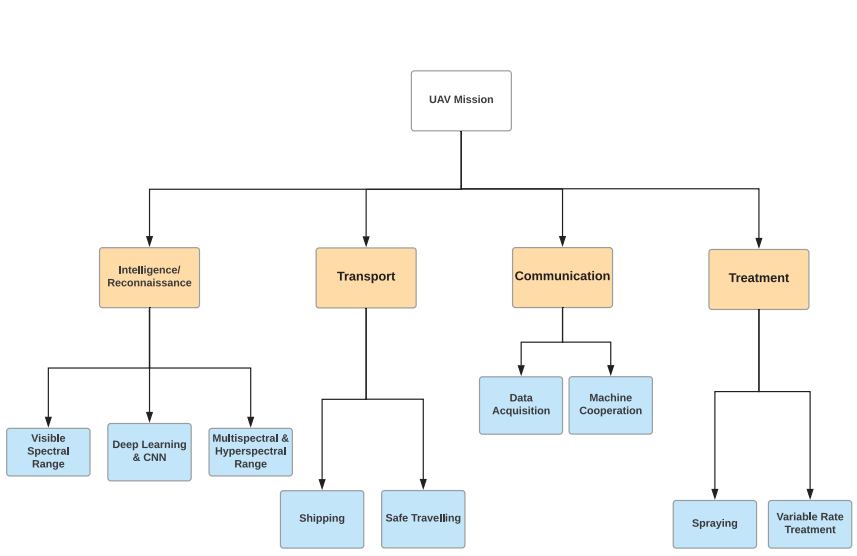
\includegraphics[scale=.7]{Drone_Groups.png}}
\caption{Classification of Drones in PA \cite{Bacco_Smart_2018}}
\label{dronegroup}
\end{figure}

\begin{figure}[htbp]
\centerline{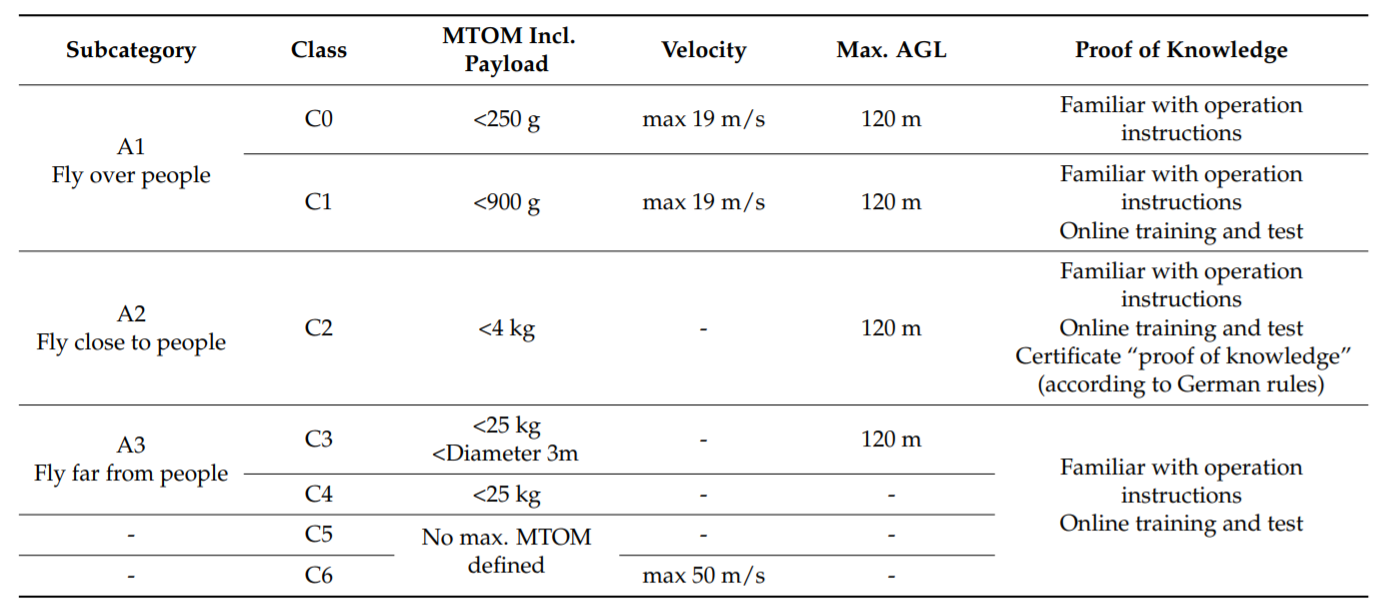
\includegraphics[scale=.5]{Drone_Safety_Categories.png}}
\caption{Category types of various UAS \cite{alamouri_exploratory_2021}}
\label{categories}
\end{figure}

\begin{figure}[htbp]
\centerline{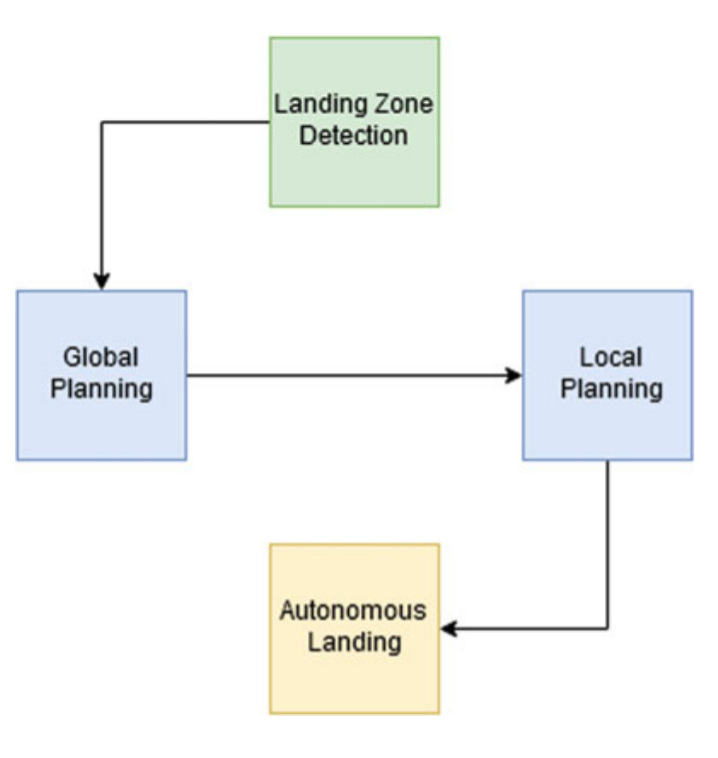
\includegraphics[scale=0.7]{UAV_Landing.png}}
\caption{UAV landing system \cite{koubaa_robot_2021}}
\label{uavlanding}
\end{figure}

\begin{figure}[htbp]
\centerline{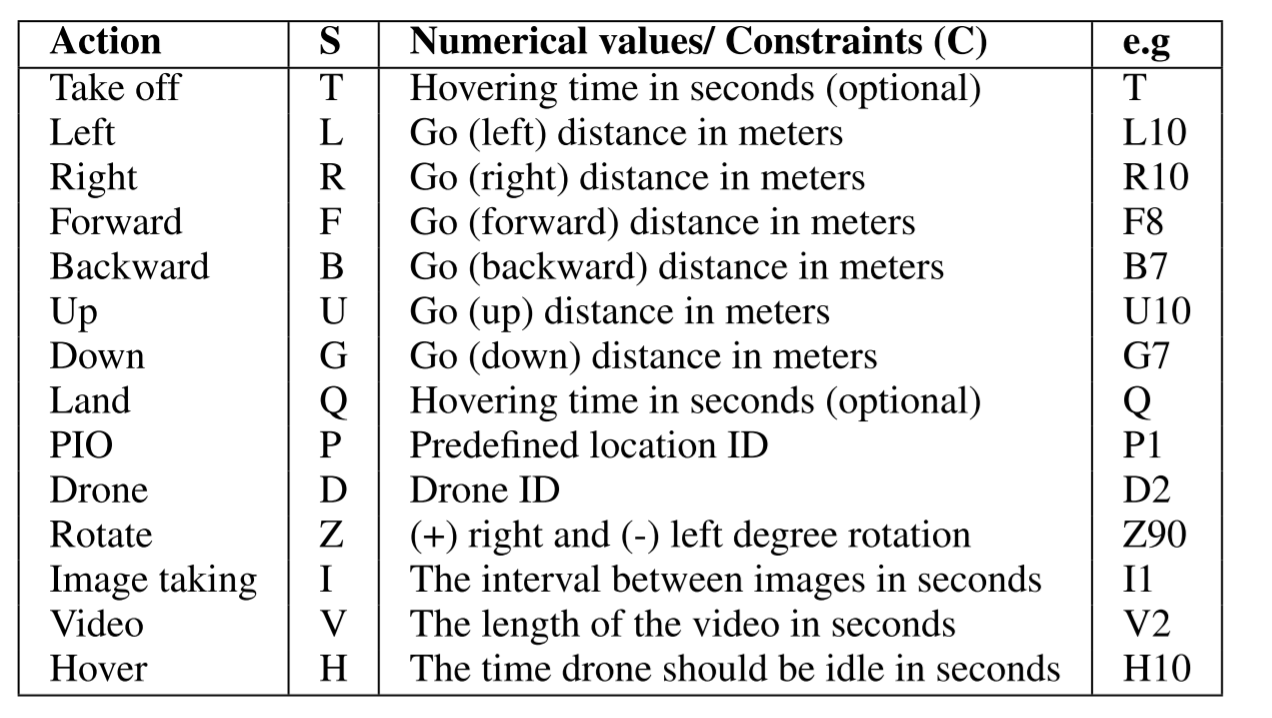
\includegraphics[scale=0.5]{DroneScript_Variables.png}}
\caption{Table of basic actions possible with DroneScript \cite{alwateer_enabling_2019}}
\label{dronescript}
\end{figure}

\bibliography{references}
\chapter{Affidavit}
I, Vytaras Juraska, herewith declare that I have composed the present paper and work by myself and without use of any other than the cited sources and aids. Sentences or parts of sentences quoted literally are marked as such; other references with regard to the statement and scope are indicated by full details of the publications concerned. The paper and work in the same or similar form has not been submitted to any examination body and has not been published. This paper was not yet, even in part, used in another examination or as a course performance.
\end{document}
